\chapter{Implementation}

\section{Location Based Help}
Throughout the design phase of the project the Help Activity is referred to as most likely to be the easiest feature to implement, when it came to implementation these assumptions were mostly correct.  Due to past work the developer was already aware of the Great Circle function\cite{circle} which saved some time.

There are a fair amount of changes to the implementation shown in the class diagram, some of this was done to simplify the process and stop code being used twice in two different places. The largest change is that the $calcDist$ function shown in the diagram has been pulled into its own class, this was done due to the route plotter also needing a function to calculate distance, it was best practice to only have the code exist once in the application.

Another change is the removal of the $loadHelpPoints$ function, while loading from a file is completed throughout the application in this case problems arose which made the process seem to be a waste of resources. While looking for information regarding people who could be contacted for help, little turned up. Details relating to three buildings were found so for the current iteration they are hard coded. 

A small change within the program is also what the $sortHelpPoints$ function returns, in the diagram it returns the sorted array. However in actuality it now returns the index of the closest location, this removes some stress on the device and is overall simpler yet still effective. A further small change is the removal of the $displayClosest$ function. In actuality this was not needed, all methods are called in the $onCreate$ due to the simple nature of the task, once the right index has been found what the method was meant to do just took a single line of code so the inclusion of this method was seen as unnecessary.

The location based help function was actually simpler than initially thought, due to its very small size. A users location is easily found using the Location Manager and from there its basic object manipulation mostly. Implementing the great circle function took some time until a fitting one could be used, taken from Stack Overflow\cite{circlef}. Other proposed solutions seemed overly complex for what was being considered.

\subsection{Updating Help Location}
One idea that was experimented with was having the activity update when it moved into a new 'area' of help. This was done by repeated updating of the user location and rerunning of the methods which calculated the closest position. While it works in practice the major issue was what was seen as a good degree of uncertainty in the calculations.

While the Great Circle function works well, with its results being tested against measurements completed on Google Maps, reliability of the GPS co ordinates were not as certain. While co ordinates give us a very close estimate of our position, they are not always perfect. After some research it was clear that civilian GPS while in good conditions could return results within a metre\cite{gps}, other factors that affect the accuracy are present on campus. Looking at figures, most GPS queries return accuracy to within 3.5 metres\cite{accuracy}. However the impacting variables of receiver quality and signal blockage are not something we can plan for, due to these reasons a series of decisions were made.

As seen on the official GPS site\cite{gps}, with the boundary between some buildings being so small, an error of 5 or so metres, something that has been seen, would provide false readings. Due to this the implementation of updating values on the Help page was omitted, the text displayed clearly displays the building the help is for, if this is wrong  a button to update values has been included.  

\section{Building Display}
During implementation a large amount of change was made to the way that the Building Display worked, a lot of this was down to it sharing an Activity with the Route Plotter. Initially this was done as the activities used similar resources and seemed small enough to not cause too many issues. However into development it was decided that the two activities really should have been separate, if nothing else than for clarities sake. However this was not decided until the features were complete, so as the project stands the screens have not been split. 
\subsection{Removal of Render Functions}
In the program the largest change is the removal of the $renderPlotter$ and $renderDisplay$ functions. In past documentation these were said to be the methods that would actually render what was needed, however these have been removed and the problem handled in the $onCreate$. This is done by the press of either the Building Display Button or the Route Plotter button initially sending through a string which represents the users desire. From there the $onCreate$ is split, if the user has said they want to plot a route then a different part of the method is entered, in both cases the visibility of a set of buttons and other interactive elements is set. By doing this we can view the activity as having two $onCreate$ methods, its just that they are nested within the same parent method. 
\subsection{Other Changes}
A change seen previously is the removal of the $calcDistance$ function from this class as well, it now relies on the class that handles all of the distance algorithms. A similar change is the removal of the $loadPlaces$ function. Loading of places is handled by the actual Place class, called locations in the application. By being moved away we keep the code in this class purely related to the displaying of locations, removing any blur between the classes. $showByType$ is implemented in the suggested way by the class diagram, it is called using the $setOnClickListener$ functions used in the $onCreate$ function. These listeners set the behaviours for an interactive element in the design, in this case the $showByType$ function is called with the buttons type being passed in as the string variable. For showing Lecture Buildings the String Lecture is passed in and the array searched for any location that matches. $showByType$ was actually initially implemented in each $onClickListener$, while no real problem for the user it meant the method was implemented for however many types of building there were. When the design was finally adhered to it vastly simplified the process and created a much better class in terms of code quality. This also means that in the future any addition to the type of buildings will only need a few lines of code instead of the repeated fifteen or so which were initially being used. 

Throughout development other applications and documentation were reviewed which showed the use of custom markers for buildings, due to this the feature was also included within the application.

\section{Route Plotter}
Route plotting was an area in the application where a fair amount of issues arose during implementation, while the feature was successful many hard decision had to be made and the result of those will have to be tested. With once again using GPS co ordinates for the positioning, problems arose with accuracy and exactly how a user would want to plot a route. Most of the class diagram relating to this feature is correct, the only difference is the movement of the log point method into the $onClickListener$.
\subsection{Plotting of points}
Plotting of points is an area which had similar issues to the updating of values in the Help feature. Mainly the testing of automatic point logging, this turned out to be a much bigger problem than in the help section. With the error in GPS co ordinates sometimes being over 3 metres\cite{gps} the automatic logging of points is not something which could be trusted to return viable results. Tests using automatic logging returned results, which when visualized, returned results similar to below. Any stop in a users movement would cause problems as any change GPS made would then cause a small difference meaning that it looked like the user was taking an erratic route.
\begin{figure}[H]
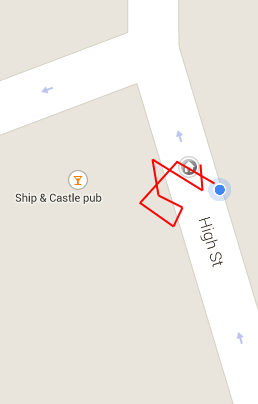
\includegraphics[scale=0.5]{Chapter3/erratic.png} 
\caption[Erratic Route Display]{Example of issues posed by automatic logging of points when route plotting}
\end{figure}
As can be seen from the pictures above this was not an ideal way to implement the feature, what is now done is a point is only added when a user asks. Having the feature implemented this way means the user is free to explore paths, yet not plot them. Providing what is seen as a more user friendly experience. Another benefit found was that by using the Google Maps $setMyLocationEnabled$\cite{setlocation} the user would be able to see their position, however the benefit goes further than that, in locations with good signal the point is plotted exactly at the displayed position. It is thought the reasoning is that both Google Maps and $logPoint$ method are both using a Location Manager which will always return the same results to both as its running on the same device.
\subsection{Visualizing and Cancelling}
Visualizing a route was implemented in the way detailed throughout the application, poly lines are drawn between each consecutive point causing a route which displays the users position throughout. Within the application every time a point is logged, except for the first time, the $paintRoute$ function is called, it takes the latest and previous logged point and simply paints a line between the two.

An implemented method which was not expected to be within the class is the $showDialog$ method, this is run when the user wants to cancel a walk. Absence of this method in the class diagram and other specifications is due to what was a lack of research on the possibility of a dialog box. It was wrongly assumed that the displaying of one would be smaller than it actually is, however the method is fairly simple. On the user wanting to cancel a walk, all points are wiped and the map cleared, on choosing no nothing is done.

\subsection{File Saving}
Saving the plotted route to a file was a task which took much longer than expected, this was due to a misread of the documentation. Through research it was found that an Android device typically has two types of storage, internal and external. It was assumed that external storage would only be possible with an SD card in the device, this was the first mistake which caused the long delay. A second compounding error was the assumption that saving to the internal memory would make the file accessible by the user\cite{storage}, something which is only possible in cases where a device is rooted. These compounding factors caused the process to take a length of time which simply was not expected and set the development off by around two working days. 

During this time it was assumed that the file was simply not being created, however in actuality it was, it was just not available through any file browser, only through the application itself. This was due to the assumption that internal memory was accessible by anyone at any time, in reality files saved by applications to internal memory are only available to that application. Due to this, looking through the file system for the relevant folder was of no use, it was there but hidden. To combat this various techniques were researched of saving files without having to rely on an SD card as not all users would have them. 

One possible method was has been mentioned before was the uploading of a route so the user could retrieve it from any web connected device. Legacy code from previous projects was used to send a JSON which included all of the relevant file information, using the LogCat feature in the Android Studio IDE\cite{as} showed that the data was being sent out, so the development could continue.

However, with further reference to some Stack Overflow answers to relevant questions\cite{check}, it was discovered that external memory is a fairly inaccurate name for what the memory actually is. In reality external memory represent one of two things, that an SD card is present or the device in question has inbuilt memory to store files\cite{storage}. With this discovery the viability of storing files locally vastly improved. As most devices are present with one or the other the final decision was that saving to external memory was the solution. With Google themselves trying to set the trend of removing the necessity of SD cards in Android devices it should be a smart decision for the future as well. 

\subsection{Writing to File}
Implementing this feature was simple once the problem of saving a file and accessing it were resolved. This functionality is provided by the $printFile$ method. This method takes the Route object and uses its variables to print a file that represents the route plotted. It is printed in such a way that it is compatible with the route finding side of the project. 

Printing the file is done with an $outputStreamWriter$ which takes a String and prints it into the file, each time a $write$ is called the writer uses a new line. Formatting for the file is as follows
$Start$\\
$Destination$\\
$Grading$\\
$Number of Points$\\
$Points$\\
$Destination$\\
$Grading$\\
$Number of Points$\\
$Points$\\
The format was dictated during the development of the route finder, having the file formatted as such allows for an easy implementation of a file reader. With the first 4 lines being static throughout files and the next being decided by the fourth line the code is easy to implement. From there we can see that another destination is listed, the above file contains details on a Node which connects to two others and the path between them. 

Once the file is saved it is up to the user what they wish to do with it, this could range from testing of a path to full implementation into the graph. While a printed file links a Node into the graph, changes still need to be made to detail the path to the Node for the use of other Nodes. This means changes need to be made to at least one other Nodes file for the Node to be fully linked. While this is not ideal there are very few ways around it, one possible way considered was to also create another file for the place the path connects to, which would contain the new path. However if multiple new paths were implemented at once, each time the new file for the Node would differ, addition by hand is not ideal but at least lets the user keep track of which files need what adding to them. 

\section{Route Plotting}
Route plotting was the key area of the application, this was due to the poor implementation of it in the original Access Aber\cite{aa}. With so much feedback from the original version it was easy to set out a set of guidelines, some of which have been mentioned in the previous Design Specification. To begin with in the implementation phase a set of guidelines were set out which, if met, would cause the feature to be seen as a success for the current time line. 

\begin{itemize}
	\item 1 - Adapt the Route selector to be two selectors, a start and destination, rather than one which contains all possible routes.
	\item 2 - Implement an extendible graph that represents the campus and building locations.
	\item 3 - Have the route display gradings for the route, if the route is in segments display each segment in its respective colour.
	\item 4 - Give the user the opportunity to take a route with no steps, ideally this would be done on the same graph as standard route finding if possible.
	\item 5 - Display basic information about the route, stairs and distance ideally.  
\end{itemize}

These five criteria were seen as fairly reasonable targets, with the only worrying task being the no step feature, something which was assumed to be difficult. Item 5 was seen as a stretch goal as it would require the editing of the file format and as such a fairly large amount of code from some small prototypes and the route plotter.
\subsection{Route Object}

Initial development time was used to implement the route object, something fairly simple. As an object itself the Route contains the information relating to its start, destination and the points along the route. This means it contains an Array List of what are called locations in the application, labelled places on the class diagram. This implementation provides us with all of the information needed to find a path through the graph. When a Node is analysed, what is really happening is that a file is being loaded in which creates a set of routes, each are checked for where they end. If the route ends at the right place the solution is found, if not its end place is added as a Node to be searched next. 

Paths between nodes are stored as a set of locations, this is an object used repeatedly throughout the application, a 'locations' object contains a range of information, most importantly the co ordinates of the point. For route finding the rest of the information possible is irrelevant, other variables are used elsewhere. Having this one object which describes a location was a real benefit during development, it saved creating classes for what were meant to be different types of location like buildings. Due to this locations can have names and descriptions, it is just that they are not important for route finding. 

\subsection{Implementing Graph}

Throughout development a range of issues were encountered, one which changed the layout of the application was where files could be opened from. Access to the $Assets$ folder which is where the files are stored is only given to Activities within the application, near the start of development the desire was to move the route finding out of the Activity and into their own class, this still would have been possible but would have caused code that solves the same problem to be split up through two classes. This was an unwanted confusion, due to it all route finding is now done in the route display activity, having been moved from the Route Choose Activity. 

Each file loaded in represents a Node and the connections to the other Nodes around it. By loading in the whole assets folder it would be possible to visualize the whole graph and the connections. One of the key problems encountered when implementing the graph was that once the search was complete, which will be discussed further on, routes would often double back on themselves as that's just how the Nodes were set up. After some research on how others had implemented representing real world maps as a graph it became obvious why.

In road travel there are decisions to be made beyond locations, routes are not planned from location to location which is what was currently being done. Junctions have to be considered when implementing a representation of the real world, these became known as 'Points of maximum traversal' throughout development. These points were where a majority of paths would have to pass through, implementing them stopped the double back issue. Campus mostly consists of some key roads, mainly the one which contains IBERS, Edward Llyd and the entrance to the Llandinam building. With this in mind there weren't too many junctions which had to be implemented, the two key junctions of travel are the area around the Students Union which links to both Hugh Owen the Union and further on most accommodation as well as the junction at the bottom of the hill, a point which most routes pass through. This connects to the row of buildings where most lectures take place as well as the sport facilities and the National Library. An issue junctions also resolved was with routes doubling back on themselves, while the route was found the representation of the real world was poor so the resulting route was also inherently poor. The issue is represented below.

\begin{figure}[H]
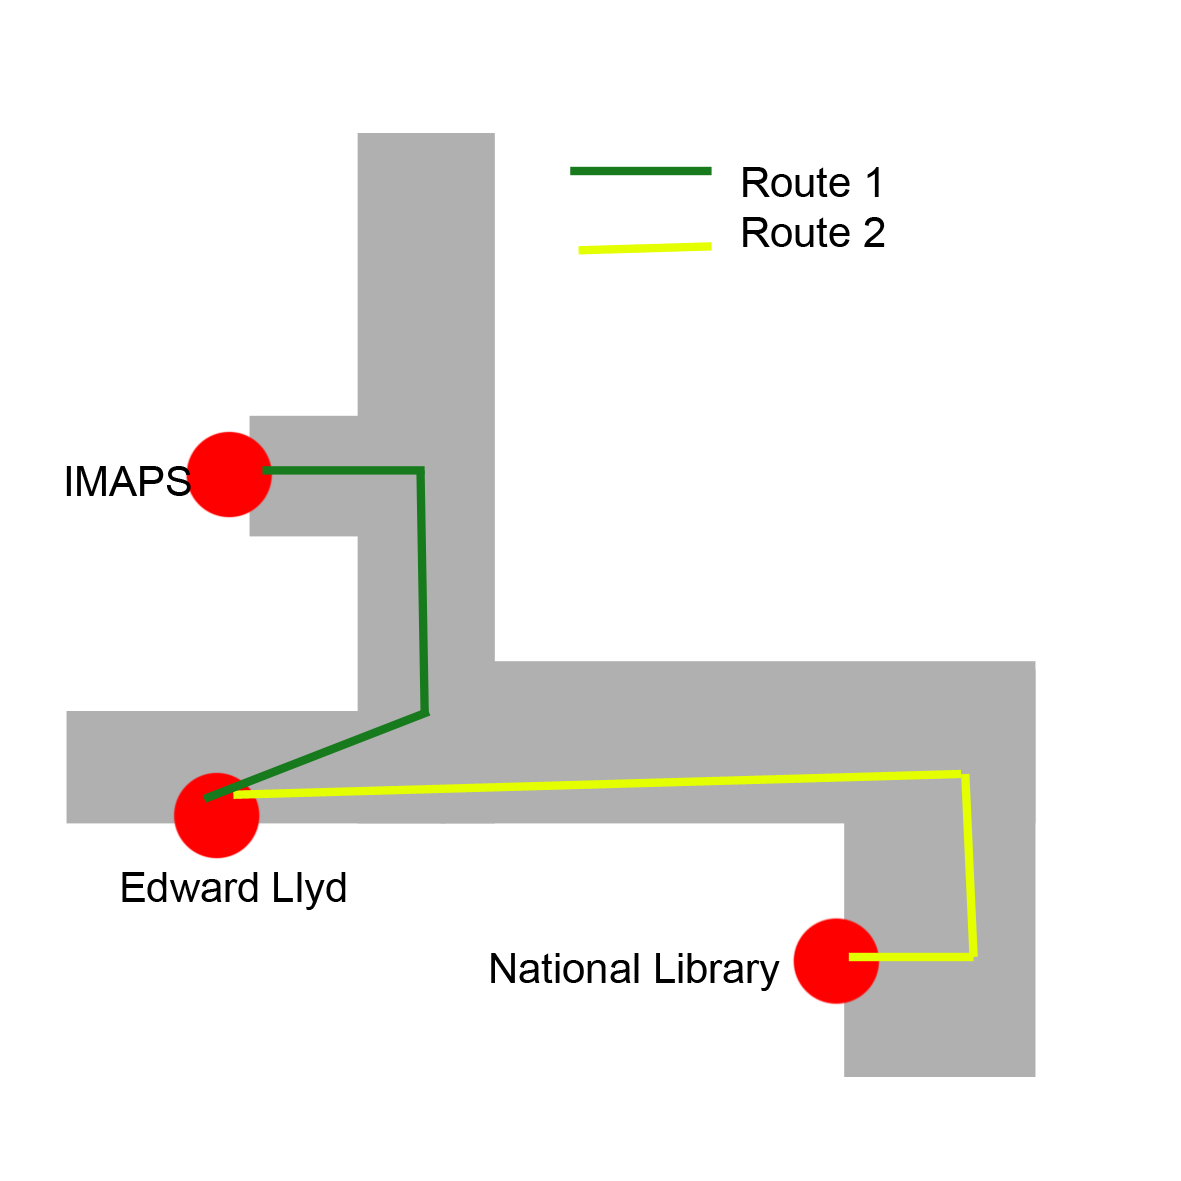
\includegraphics[scale=0.5]{Chapter2/beforepomt.png} 
\caption[Route Before Junction]{Example of route issues caused by the lack of junction consideration in the graph.}
\end{figure}
\begin{figure}[H]
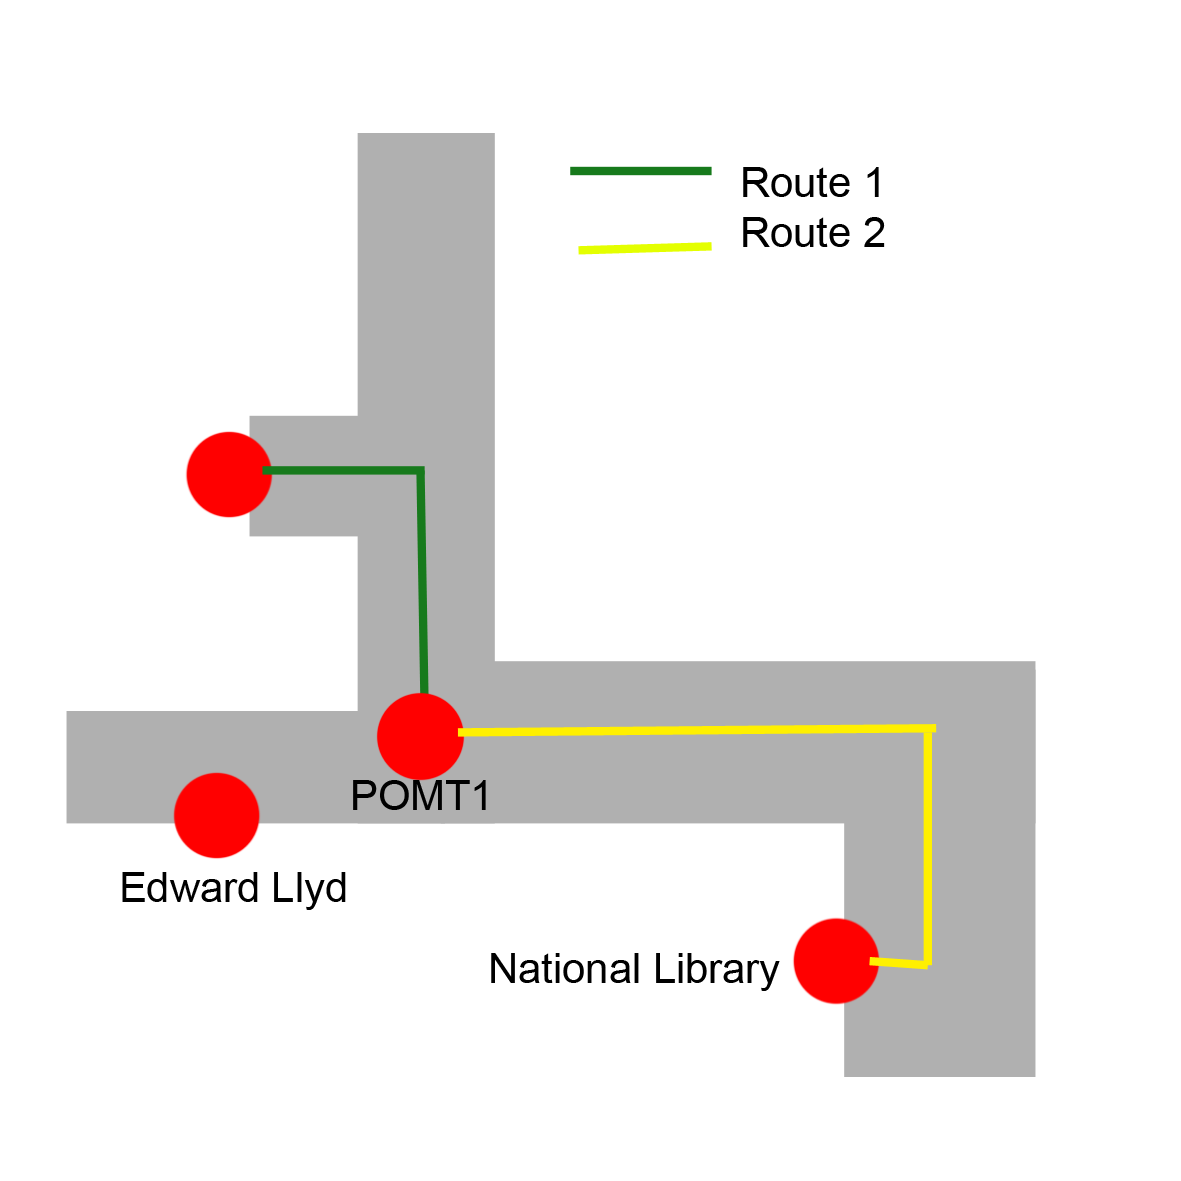
\includegraphics[scale=0.5]{Chapter2/pomt.png} 
\caption[Route after Junction]{How the consideration of junctions improves route finding through a more accurate representation.}
\end{figure}

\subsection{Step Free Graph}
Implementing the step free graph was a fairly simple process in its current version, though it is an area that could do with improvement. Currently upon a user asking to find a route they are asked if they would like their route to be step free, if so the same activity is loaded but the route finder logs that the user wants a step free route. By doing this the user has essentially set which graph will be used. Currently the step free and standard graph are completely separate, contained within two folders nested in the assets folder. During searching the algorithm uses a keyword passed in to determine the folder files are being fetched from. This applies to the expandable list views in the route choosing activity as well. In future it would be beneficial to have one consolidated graph, including full route information and different routes between the same points allowing for path finding with variables.  
\newpage
\subsection{Search Algorithm}

Initially fairly little research was done on how to build the search algorithm, throughout documentation it had been referred to as a Breadth First Search but when it came to implementation it was thought that creating any search would be a good base to build upon. However it quickly became obvious that what was being attempted was a BFS\cite{bfs} and as such references should be made on how to implement it properly first time. A large amount of delay came from implementing the Search algorithm as not only was it a search, it was a plotting of a set of routes and representation of them on the Map object. 

After the basic search algorithm had been implemented the initial issue was a lack of tracking the path that was moved through, this was down to not implementing the Node class shown in the Class diagram. In the class diagram the Node objects represents each file opened and where it was opened from. By logging these it was then possible to track back from the destination Node to the start. A Node is added when it has been checked for two things, first that it has not been previously visited and secondly if its is not already in the queue to be visited. This stops the duplication of paths to Nodes being considered when following the route back. All that was being returned to begin with was the final route found, so the destination and the Node that opened it.

In development this was the first issue to be fixed, currently the algorithm finishes its run through and goes back through the graph, moving from a Node to where that Node was opened from. While doing this it passes the start and destination back to the algorithm which starts the search, however the search does preliminary checks to see if the route is already stored in the start Nodes file, meaning the two are already directly connected. This is guaranteed to be true in this case so the actual BFS is never hit. From there the Route information is passed on to the paint function. 

\subsection{Painting the Path}
Painting the path was an area were little changed from the planned design, it is near identical to the imagined solution. To paint the path a Route object and the Map object are taken as parameters, a loop is completed through the points along a route, a line is painted between the two points by turning them into $LatLng$ objects which are used when painting a poly line. To accommodate the grading feature the line is painted in its respective grading using the $parseColour$ function provided. This continues until the last point where the function stops to prevent crashing. While simple no improvements could be thought of regarding the method, some visual improvements were considered including a fading of colour between segments however a solution could not be found. 

\section{UI Design}

\subsection{Map}

Implementing the map feature was a fairly easy process, once the relative keys were set up and the correct package approved in the API console. One major decision throughout the process was the type of map that would be appropriate in each activity. Throughout the application the map differs based on what the user is doing, if they are trying to find a building the map gives an abstract representation as it is all that is really needed. If a user is route finding then a photographic representation is give. This can be changed in future and is another possible area for user testing. 

\subsection{Relative Design}
Designing in such a way that an activity adapts to its screen was a task that was incredibly time consuming compared to what was expected. This is put down to the fact that the developer had little experience with XML and how to use it to be most effective. Despite this Android Studio provided a range of features which provided great assistance causing a quicker rate of development in the closing stages of the project.

One of the main problems was finding a menu layout which could be made to be adaptive to any screen, it was decided that a grid layout was a good option as no matter what we should be able to split a screen into the four possible functions. Early on research was done into the $GridLayout$ however it required API level 14, it was felt the application could be developed to a lower point than this. Due to this a way had to be developed to have the grid work.

This was achieved through the use of fake views, these were view objects with no height or width on the screen, by including these it was possible to align buttons around them. From there setting buttons to fill their possible space was easy. Further problems arose with using white space around the buttons, something set out in the Design section. With issues in padding and margins not working, for still unidentified reasons it was necessary to resort to the graphical editor provided. With this the changes were made in minutes, while learning what can be done with  XML it was also important to make best use of the tools available as the feature was closing in on taking too long for the benefit it would provide. A representation of fake views can be seen below. 
\begin{figure}[H]
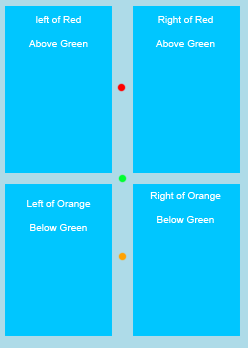
\includegraphics[scale=0.8]{Chapter3/fakeview.png}
\caption[FakeView Example]{An example of using fake views for alignment, buttons are set to be a specific side of the view.}
\end{figure}
Custom buttons were one of the least complicated features within the application, the facilities provided by Android were far from perfect, with some researching it was noticed that the best solution would just be custom buttons. In this case the application makes use of an adapted on line resource\cite{button}, with the base code being taken from the site and edited to fulfil the developers needs. 

From there the screens are fairly simple, buttons are set at the bottom of maps and maps fill the screen unless the device used is very large. With some testing already done on various screen sizes it is fair to say an adaptive design has been achieved. UI implementation was by far the most underestimated task throughout the project design, at times it set the project far behind schedule. 
\section{Conclusion}
To conclude the current achievements will be referenced to the functional requirements (FR) set out in the requirements specification section 4.1.2 in this document. Moving through the FR's it is possible to see most of the requirements have been met, with some missing but other alternative implemented. In the list set out the first requirement is the Route finding function, further detail provided specifies the use of colour coded routes. This has all been achieved while maintaining a high level of extendibility including menu portions and the graph itself, this can be considered a strong success. One area for improvement however would be the improvement of displaying information along a route. 

FR2 was a location based help service, that gave the user a person who could possibly help them. While this has been met it is by far the functionality which has the most room for improvement. While implemented to what has been stated it is felt to still be fairly underwhelming compared to the feature it could be. An area where future work should be heavily considered.

FR 3 was the ability for a user to display buildings, filtering the type. Another are which can be considered a success, partly down to the simplicity of the functionality. It is further highlighted in the specification that the locations should be loaded from an easily update able file, another implementation. From there further modifications were made, including information on the buildings department requested from the previous feedback form and custom markers, small but adds some difference to the application. 

FR 4 was to implement a route plotter for the user, including the grading of the route. Another feature fully implemented, not only can a user plot a route but they can visualize what it will look like in the route finder as well as log the steps on the route and have the distance logged for them. A file is also output for the user to do with as they wish, with the file being fully compatible with the route finder. Another functional requirement fully met, possibly exceeding initial expectations.

FR5 was a feature which was possibly lost along the way of development due to varying issues. Mainly the lack of support for Welsh within Android. Due to this the welsh locale would have to be set programatically, an area which seems to cause issues for any who have done it previously. Due to this a test feature has been implemented, this sets the locale to French but the strings file used actually uses a Welsh translation. While a hack like implementation, it is still functional and is a proof of concept if Welsh locale is added.

A functional requirement which should have been included is a good UI design, while referenced throughout it is never seen as key, which it is now seen as after development. In the applications early development, its use was hindered by poor layout, design and flow. While this has changed considerably the memory of how badly the design effected user experience made the effort in including what is reasoned to be solid design worth it.

Overall the project is considered a success, with all functionalities being mostly met, some exceeding expectations while one or two needing more work to be the fully finished product. For the time line given the developer is satisfied with the achievement. 

 